%! program = pdflatex

\documentclass[11pt, final]{article}
\usepackage{geometry}
\geometry{letterpaper} 
\usepackage{cite}
\usepackage{fancyhdr}
\usepackage{graphicx}
\usepackage{asymptote}
\usepackage{verbatim}
\usepackage{moreverb}
\usepackage{multirow}
\usepackage{setspace}
\usepackage{cprotect}
\usepackage{enumerate}
\usepackage{amsmath}
\usepackage{titlesec}
\usepackage[labelsep=period, bf, singlelinecheck=false]{caption}
\usepackage[title]{appendix}
%\usepackage[T1]{fontenc}
%\usepackage{times}
 
\pagestyle{fancy}
\renewcommand{\headrulewidth}{0pt}
\textwidth6.5in
\oddsidemargin0in
\topmargin-.75in
\headheight.5in
\headsep.125in
\textheight9in 

\def\verbatimtabsize{4\relax} 

\titleformat{\chapter}[display]{\vspace{0.3\textheight}\normalfont\huge\bfseries\centering}{\chaptertitlename\ \thechapter :}{20pt}{\Huge}
\titleformat{\section}{\LARGE\bfseries}{\thesection}{1em}{}{}
\titleformat{\subsection}{\Large\bfseries}{\thesubsection}{1em}{}{}
\titleformat{\subsubsection}{\large\bfseries}{\thesubsubsection}{1em}{}{}
\titleformat{\paragraph}[hang]{\normalsize\bfseries}{\theparagraph}{1em}{}{}

\renewcommand{\labelitemii}{\(\circ\)}

\lhead{}
\chead{}
\rhead{}
\lfoot{}
\cfoot{}
\rfoot{\thepage}

%%% BEGIN DOCUMENT
\begin{document}
%\maketitle
\doublespacing
\setcounter{secnumdepth}{4}
\begin{titlepage}
\center

\hspace{0.5in}\\
%\vspace{0.75in}

\huge
\textbf{Design Proposal for Robotic Wall Following Technique Using Ultrasonic Sensors}\\

\vspace{0.75in}

\LARGE
Christopher Hood\\
Stuart Kent\\
Matthew McGraw\\
Anya Skomorokhova\\
\hspace{1in}\\


ECE 2031, Digital Design Lab\\
Section L06\\
\hspace{1in}\\

\Large
Georgia Institute of Technology\\
School of Electrical and Computer Engineering\\

\vspace{1in}

\large 
Submitted\\
November 21, 2011\\

\end{titlepage}

%\begin{abstract}
%Hello!
%\end{abstract}

\section{Executive Summary}

An SCOMP wall following program was designed for the Amigobot
using sonar feedback to determine what velocity commands to send to
each wheel. This program enables the robot to locate and travel
parallel to a wall with inner and outer corners of \(90^\circ\). The
solution to this challenge is a state machine program that executes
commands based on the current state and the measured distance to the
nearest wall. The state machine consists of four states: ``forward
motion,'' ``inside turn,'' ``adjust outward,'' and ``adjust inward.''
In ``forward motion,'' the robot moves forward full speed until it senses a
wall in front of it or no wall is sensed. If a wall is sensed in front
of the Amigobot, the program switches to the ``inside turn'' state,
turns \(90^\circ\), and then proceeds to travel forward. If no wall is
sensed, the Amigobot will adjust inward until it is parallel to the
wall, and then continue on a straight path. A switch is used to toggle
between following a wall on the left side or on the right side of the
robot. The switch position determines turning direction and selects
the ultrasonic sensors used to measure distance to the wall. Parallel motion to
the wall is maintained by switching to ``adjust outward'' and ``adjust
inward'' states, which correct the robot trajectory if the measured
distance is not within an acceptable range of \(20\pm1\) cm. Inputs to
the state machine are ultrasonic sensory data. The outputs are
velocities of the left and right
wheels. During the final demonstration, the robot running this program
was moderately successful in following the test course. It
successfully navigated the wall on the right side and received an
accuracy bonus. While the robot completed the course when following
the wall on its left side, it did not receive an accuracy bonus and
did not finish the course in the desired time frame.



\section{Introduction}
\subsection{Design Problem}
The goal of this project is to design an SCOMP wall following program
that enables the Amigobot to follow walls. The design solution meets
the following specications:

\begin{enumerate}
\item Use an eight bit velocity command where \(+127\) (\verb+0x007F+)
  is full speed forward, \(-127\) (\verb+0xFF81+) is full speed
  reverse, and zero is stop.
\item Control position by reading the cumulative rotation counter of
  the wheel.
\item Use velocity feedback and position feedback from the wheels via
  the existing optical encoder peripheral.
\item Provide a start button to begin execution after the robot is
  placed adjacent to a wall.
\item Use existing sonar and velocity control peripherals to issue
  commands to each wheel.
\item Travel parallel to a wall at a distance of 20 cm.
\item Select by switch or recompile to follow left or right walls.
\end{enumerate}

The Amigobot was expected to navigate a course without collisions and
in a specified time frame. A sample course layout is shown in
Fig.~\ref{samplecourse}.

In addition to the required specifications, the wall following program
improved the user interface of the robot by enhancing the 7-segment,
LCD, and LED displays.

\begin{figure}[h!]
  \centering \cprotect \fbox{
    \begin{minipage}{3.5in}
      \centering
      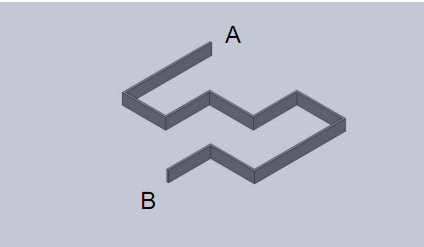
\includegraphics[width =
      \textwidth]{./graphics/course.png}
      \cprotect \caption{Sample course layout for robotic
        wall-following.}
      \label{samplecourse}
    \end{minipage}
  }\end{figure}

\subsection{Design Solution}

The SCOMP program written for the design problem is a state machine
consisting of four states. In the ``forward'' state, the
robot follows a straight trajectory until it senses a wall in front or
no wall is sensed. If the Amigobot senses a wall in front of it, the program
switches to the ``inside turn'' state, turns \(90^\circ\), then proceeds
on a straight trajectory. If no wall is sensed, the Amigobot adjusts
inward until it is parallel to the wall. The two adjustment states,
``adjust outward'' and ``adjust inward,'' maintain parallel motion to the
wall by correcting the robot trajectory when the measured distance to
the wall is not within an acceptable range of \(20\pm 1\) cm.

A switch is used to toggle between following a wall on the left side
or on the right side of the robot. The switch position activates the
ultrasonic sensors on one side of the robot and determines clockwise
or counterclockwise turning direction.

The initial approach discussed in the proposal (see
Appendix~\ref{proposal}) implemented an
additional ``outside turn'' state. During testing, it was discovered
that the state causes the robot to turn prematurely and collide with
the wall whenever the robot was not parallel to the wall. To overcome
this challenge, the team used the ``adjust inward'' state to make
incremental turns around an outside wall corner.

Additionally, the initial design called for one sensor reading from
the lateral region of the robot and one from the forward region of the
robot. During
testing it was discovered that accuracy in maintaining the set
distance improved when the minimum value of two sensors in the lateral
and forward regions were used as inputs to the states.

The role of the LCD display had to be altered when the team ran into
issues of consistency. The LCD display was initially expected to show
the moving state the robot is in. Due to the display not working
consistently, it was changed to show the basic startup states.

The design demonstration met most of the specifications outlined
above. The robot successfully completed the course for both the left
and right sided walls. It received an accuracy bonus for maintaining
the desired 20 cm distance when following the right wall. However, it
was unable to earn the accuracy bonus when following the left wall.

\section{General Methodology}

\subsection{Process and Sensor Description}

The wall following algorithm implemented follows the process found in
Fig.~\ref{flowch}. 

\begin{figure}[h!]
  \centering \cprotect \fbox{
    \begin{minipage}{3.5in}
      \centering
      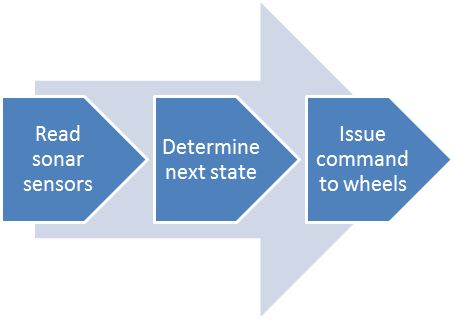
\includegraphics[width =
      \textwidth]{./graphics/flowchart.png}
      \cprotect \caption{Flow chart of wall following algorithm.}
      \label{flowch}
    \end{minipage}
  }
\end{figure}

A switch is used to toggle between following the left wall and
following the right wall. The value of the switch determines which sensors are actively
collecting data. The values of the following sensors will be used:

\begin{itemize}
\item Minimum value of sensors \(s_4\) and \(s_5\) (\(s_0\) and
  \(s_1\) for left-wall following):
  \begin{itemize}
  \item Measure the distance to the closest parallel wall
    (Fig.~\ref{s0s1}).
  \end{itemize}
\item Minimum value of sensors \(s_2\) and \(s_3\):
  \begin{itemize}
  \item Measure the distance to an approaching wall (Fig.~\ref{s2s3}).
  \end{itemize}
\end{itemize}

\begin{figure}[h!]
  \centering \cprotect \fbox{
    \begin{minipage}{3.5in}
      \centering
      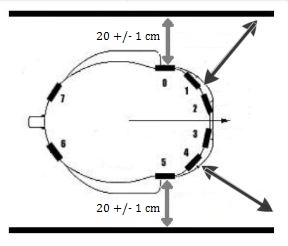
\includegraphics[width =
      \textwidth]{./graphics/s0s1.jpg}
      \cprotect \caption{Sensors \(s_4\) and \(s_5\) (or \(s_0\) and
        \(s_1\)) measuring distance to wall.}
      \label{s0s1}
    \end{minipage}
  }
\end{figure}

\begin{figure}[h!]
  \centering \cprotect \fbox{
    \begin{minipage}{3.5in}
      \centering
      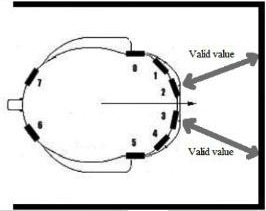
\includegraphics[width =
      \textwidth]{./graphics/s2s3.jpg}
      \cprotect \caption{Sensors \(s_2\) and \(s_3\) 
        measuring distance to front wall.}
      \label{s2s3}
    \end{minipage}
  }
\end{figure}


\subsection{State Machine Description}

The description of the states is listed below. The UML state machine
diagram the team used to implement a solution is found in
Fig.~\ref{state}.

\begin{enumerate}
\item \textbf{Forward:} The robot moves forward alongside a
  wall. A tolerance of \(\pm1\) cm is used to keep the robot in a
  range of 19-21 cm from the wall, measured by sensors
  \(s_4\) and \(s_5\) (or  \(s_0\) and \(s_1\)).  If the distance to the
  wall is not within the specified range, the robot
  switches to one of the adjustment states, which are dependent upon
  which wall is followed.  If a wall is detected in front of the robot
  by sensors \(s_2\) or \(s_3\), the robot switches to the ``inside
  turn'' state. 
\item \textbf{Adjust Outward:} The robot veers slightly outwards to get
  back within the accepted distance range. After the robot is within
  the accepted distance range, the machine switches to the ``forward''
  state.
\item \textbf{Adjust Inward:} The robot veers slightly inwards to get
  back within the accepted distance range. After the robot is within
  the accepted distance range, the machine switches to the ``forward''
  state.
\item \textbf{Inside Turn:} The robot stops and turns \(90^\circ\) clockwise or
  counterclockwise, depending on if the wall followed is on the right
  side or on the left side. Fig.~\ref{it} demonstrates this turn when the
  robot is following a right wall and is turning counterclockwise.
\end{enumerate}

\begin{figure}[h!]
  \centering \cprotect \fbox{
    \begin{minipage}{6.5in}
      \centering
      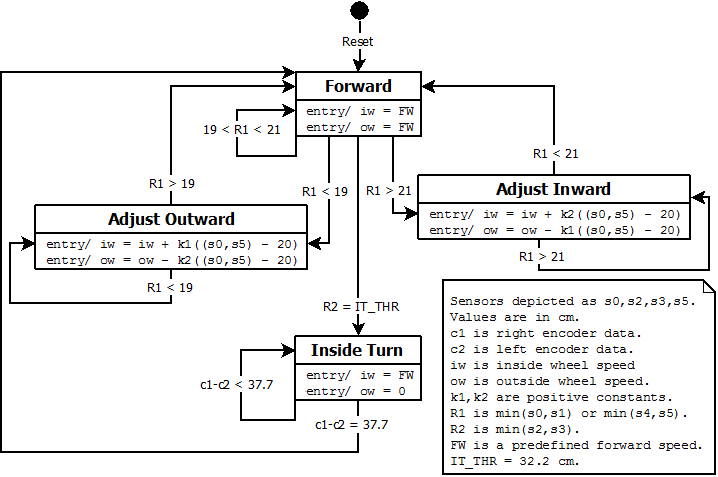
\includegraphics[width =
      \textwidth]{./graphics/smdiagram.png}
      \cprotect \caption{UML state machine diagram for wall following
        algorithm for Amigobot.}
      \label{state}
    \end{minipage}
  }
\end{figure}


\subsection{Navigating Corners}

The robot's turning algorithm takes advantage of the course only
containing turns of approximately 90\(^\circ\). Such sharp turns
are not conducive towards ``smooth'' wall following techniques.
Therefore, when necessary, the robot will execute a blind turn which relies on the
optical rotary encoders on each wheel instead of the sonar data.
The goal of the turning algorithm is not to pivot exactly 90\(^\circ\)
and then move in a straight line every time, but rather to quickly
execute a precise turn which results
in the robot being approximately parallel to and 20 cm away from the
opposite wall, after which the robot can easily continue using sonar
data to make accurate adjustments.

\subsubsection{Detecting a Turn}
The turning algorithm being implemented requires accurate detection of
forward obstacles and discontinuities in the parallel wall in order to
avoid turning prematurely.

The outside turn is not detected directly. Rather, the case of an
absent parallel wall is handled by the ``adjust inward''
state. However, the sensor values for \(s_4\) and \(s_5\) (or \(s_0\)
and \(s_1\)) must be severely limited in order to avoid having the turn 
be executed too sharply. In the program the working value for these
sensors is limited to \verb+0x0140+, or about 32 cm.

\begin{figure}[h!]
  \centering \cprotect \fbox{
    \begin{minipage}{4.5in}
    \centering
    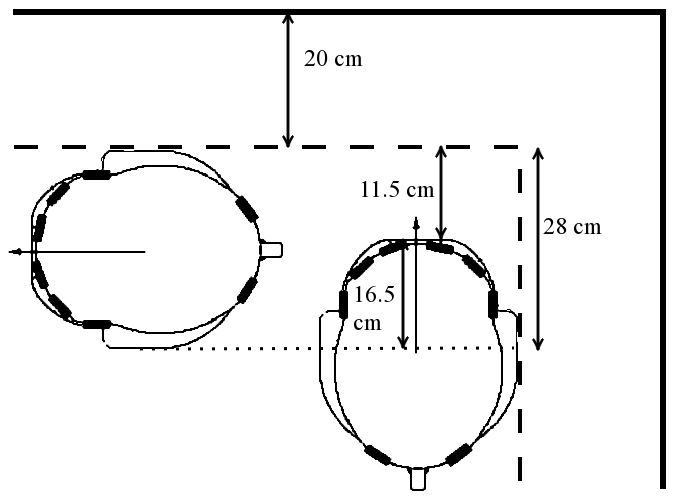
\includegraphics[width =
    \textwidth]{./graphics/inside_turn.png}
    \cprotect \caption{Geometry of an inside turn.}
      \label{it}
    \end{minipage}
  }
\end{figure}

For an inside turn, the robot must begin turning once the front of the
robot reaches the threshold \verb+IT_THR+. The geometry for this turn is
presented in Fig.~\ref{it}, which indicates that \verb+IT_THR+ should
be \(31.5\) cm. However, the forward sensors \(s_2\) and \(s_3\) are
not pointed directly forward, but rather are at \(12^\circ\) angles,
so the sensor reading for \verb+IT_THR+ should be
\(31.5/\cos(12^\circ)=32.2\) cm before the robot begins an inside
turn. The inside turn is executed by stopping the inside wheel while
driving the outside wheel forward until the robot has rotated 90
degrees (see \ref{xturn}). 

\subsubsection{Using Rotary Encoders}

The optical rotary encoders on each wheel of the Amigobot provide an
incredibly fine yet robust way to detect the rotational position of
each wheel. Each wheel's position can be loaded through SCOMP's
I/O through the I/O addresses \verb+0x80+, \verb+0x81+, \verb+0x88+, and
\verb+0x89+, which respectively correspond to the given address names
\verb+LPOSLOW+, \verb+LPOSHIGH+, \verb+RPOSLOW+, and \verb+RPOSHIGH+. The position
datum from each encoder is a 32-bit number. For I/O purposes, this datum
is split into two 16-bit numbers (the upper 16 bits and the lower 16
bits), each of which corresponds to the ``low'' or ``high'' I/O
address for each wheel's position.

\paragraph{Physical Characteristics of the Rotary Encoders}
The encoder datum increments by \(39000\) for each revolution of the
wheel. The left encoder increments when the left wheel is in forward
motion, while the right encoder decrements when the right wheel is in
forward motion. Each wheel has a diameter of 10 cm, which results in a
path of 31.42 cm being traversed for each wheel revolution so long as
traction is maintained. Since there are \(39000\) ``ticks'' per
revolution, one cm of linear wheel motion corresponds to \(1241.41\)
ticks. This results in large-valued encoder data for relatively short
distances. In order to simplify calculations and prevent bit carries
between two 16-bit numbers (the high and low data), it is best to
perform calculations on a single 16-bit number which can be produced
by combining the upper eight bits of the ``low'' datum with the lower
eight bits of the ``high'' datum, resulting in a reduction in encoder
resolution by a factor of 256.  After shifting and truncating the two
16-bit numbers into one 16-bit number, the physical characteristics of
the encoder transform so that there are \(152.34\) ticks per wheel
revolution and \(4.85\) ticks per cm of linear wheel motion.

\subsubsection{Executing a Turn} \label{xturn}
\begin{figure}[h!]
  \centering \cprotect \fbox{
    \begin{minipage}{3.5in}
      \centering
      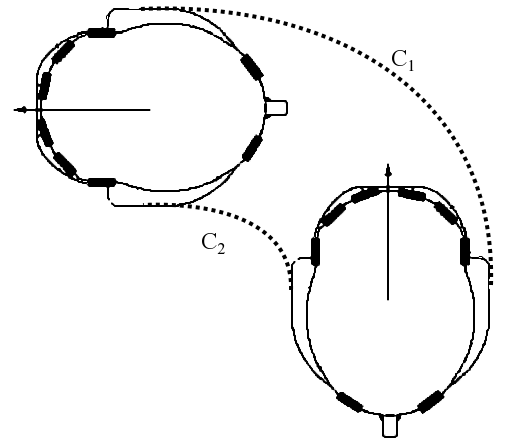
\includegraphics[width = \textwidth]{graphics/turning.png}
      \cprotect \caption{Path lengths \(C_1\) and \(C_2\) as the robot
        turns.}
      \label{turning}
    \end{minipage}
  }
\end{figure}

The linear path lengths of each wheel are related by a constant such
that when the difference in path lengths of each wheel is equal to
that constant, the robot is oriented precisely at an angle \(\theta\)
to its starting orientation. If the robot has a wheel track of \(R\)
and the linear path lengths of the right and left wheels are
represented respectively by \(C_1\) and \(C_2\) (Fig.~\ref{turning}),
then the robot has turned positive (counterclockwise) \(\theta\)
radians when the following equation is satisfied:
\begin{equation}
  C_1 - C_2 = \theta R
\end{equation}
For instance, if the Amigobot (\(R = 24\) cm) is to turn
90\(^\circ\) then continue forward, the robot should cease
turning when \(C_1-C_2 \geq 0.5\pi (24) = 37.7\) cm, or about 181
(\verb+0x00B5+) ticks. Experimentally, it was found that at higher
speeds the wheels of the robot slipped slightly when the robot
decelerated from a turn, so the working
value of this constant was lowered to 154 ticks (\verb+0x009A+).

\subsubsection{Adjustment States}

Once the lateral sensors detect that the robot is outside of the
\(20\pm1\) cm range, the robot enters one of two adjustment
states. The robot feeds back the detected range difference to the left
and right wheel velocities. 

The program uses a cumulative adjustment
where each loop iteration is paused for 100 ms. During each loop
iteration, the angular velocity for each wheel is set to a new value
based on its previous value and the measured distance to the wall, \(R_1\):
\begin{align}
\omega_i [n] &= \omega_i [n -1] + k_1 (R_1 - 20) \label{wi}\\
\omega_o [n] &= \omega_o [n -1] - k_2 (R_1 - 20) \label{wo}
\end{align}
\(\omega_i\) is the inside wheel velocity (right wheel for right-wall
following), \(\omega_o\) is the outside wheel velocity, \(k_1\) and
\(k_2\) are positive constants, and \(R_1\) is the minimum value of sensors \(s_4\)
and \(s_5\) (or \(s_0\) and \(s_1\)).


\subsection{SCOMP Alterations}

Several alterations to the SCOMP program were  made in the form of
new instructions:

\begin{enumerate}
\item \textbf{MULT} - The built-in
  Altera\textregistered~megafunction
  \verb+LPM_MULT+ was implemented into SCOMP, with the module
  multiplying the accumulator, \verb+AC+, and memory data register, \verb+MDR+. The 32-bit result vector
  for \verb+LPM_MULT+ is latched and spread across 16-bit registers
  \verb+LO+ and \verb+HI+ when SCOMP enters the \verb+EX_MULT+
  state. 
\item\textbf{MLO} - The contents of the \verb+LO+ register (the lower
  16 bits of the result of \verb+LPM_MULT+) are
  latched onto the \verb+AC+.
\item \textbf{MHI} - The contents of the \verb+HI+ register (the upper
  16 bits of the result of \verb+LPM_MULT+) are
  latched onto the \verb+AC+.
\item \textbf{DIV} - The megafunction \verb+LPM_DIVIDE+ was
  implemented to divide \verb+AC+ by \verb+MDR+. The remainder of the
  megafunction result is latched onto register \verb+REMAI+.
\item \textbf{REM} - The contents of \verb+REMAI+ are latched onto the
  \verb+AC+. 
\item \textbf{SHIFT2} - The megafunction \verb+LPM_CLSHIFT+ was
  implemented to shift by a variable amount. Instead of the shift
  magnitude being four bits of \verb+IR+ as in the original
  \verb+SHIFT+ instruction, the shift
  amount for \verb+SHIFT2+ is specified by the first four bits of
  \verb+MDR+. Additionally, in order to simplify the assembly program,
  the shift direction was inverted so that when \verb+MDR(4)+ is low,
  a right shift is indicated.
\item \textbf{SHIFT3} - A third instance of megafunction
  \verb+LPM_CLSHIFT+ was implemented in order to provide a variable
  rotating shifter. The megafunction parameters are identical to those
  of \verb+SHIFT2+ except for the shift type. 
\end{enumerate}

The \verb+MULT+, \verb+MHI+, and \verb+MLO+ intructions are used in
the two adjustment states for the multiplication required in equations
\ref{wi} and \ref{wo}. The divide instruction as well as the two shift instructions are used in
manipulating the LED displays as described in section \ref{leds}.

\subsection{Amigobot Display Additions}

Several additions were made to the robot display to improve the user
interface. Memory locations used to write to and read from are designated in capital letters.

\begin{figure}[h!]
  \centering \cprotect \fbox{
    \begin{minipage}{4.5in}
      \centering
      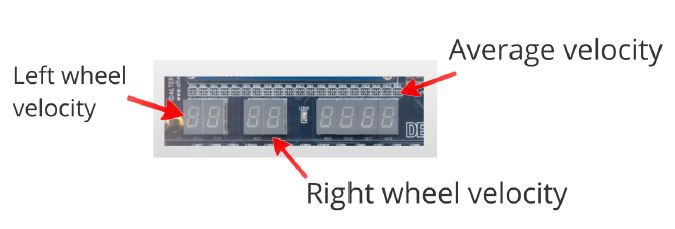
\includegraphics[width = \textwidth]{graphics/7seg.jpg}
      \cprotect \caption{Implementation of both seven-segment
        displays.}
      \label{7seg}
    \end{minipage}
  }
\end{figure}

\begin{itemize}
\item Two displays are used to show the velocity of the left and
  right wheels.
  \begin{itemize}
  \item These are written to \verb+SEVENSEG+ whenever \verb+LVELCMD+
    or \verb+RVELCMD+, the wheel velocities, are changed
    (Fig.~\ref{7seg}).
  \end{itemize}
\item The third display shows the velocity of the robot
  (Fig.~\ref{7seg}).
  \begin{itemize}
  \item This was done by altering the \verb+IO_decoder+ and the block
    diagram files so that the second 7-segment display
    could be written. It is named \verb+SEVENSEG2+ and mapped to
    0x05 on the IO address space map.
  \item\verb+IO_decoder+ was altered by adding and enabling a
    signal for the second set of the 7-segment LEDs and copying the
    setup of the \verb+HEX_DISP+ module used for the current 7-segment
    display.
  \end{itemize}

\begin{figure}[h!]
  \centering \cprotect \fbox{
    \begin{minipage}{4.5in}
      \centering
      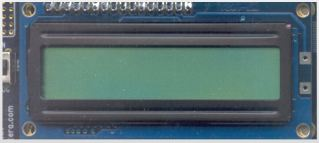
\includegraphics[width = \textwidth]{graphics/lcd.jpg}
      \cprotect \caption{The LCD display on the DE2 board.}
      \label{lcd}
    \end{minipage}
  }
\end{figure}

\item The LCD display (Fig.~\ref{lcd}) shows the current state the program is in.
  \begin{itemize}
  \item This was done by altering the LCD display to accept ASCII
    values representing numbers. The SLCD was altered to take in an
    ASCII enable, \verb+ASCII_EN+, which tells it to interpret the
    incoming argument as a state to be output in ASCII format.
  \item There are four states. The LCD displays \verb+RDY!+ when the
    program is ready to start. It then displays \verb+KEY2+ to tell
    the user to press \verb+KEY2+ and start the program. Once the
    program starts, the screen displays \verb+LEFT+ or \verb+RGHT+,
    telling the user which side of the wall the robot is following.
  \item The states were encoded into a binary code of 16 bits. For
    example, the \verb+RDY!+ output string was encoded as \verb+0x0+ and the
    \verb+KEY2+ command as 0x1. The strings shown on the LCD display
    were hard coded using the binary state representations.
  \end{itemize}

\begin{figure}[h!]
  \centering \cprotect \fbox{
    \begin{minipage}{4.5in}
      \centering
      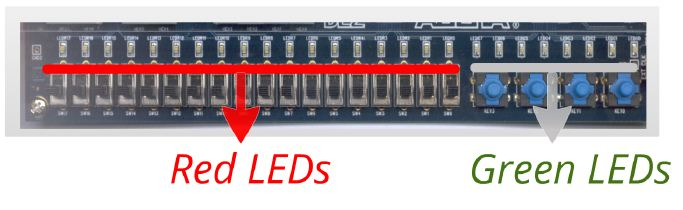
\includegraphics[width = \textwidth]{graphics/ledf.jpg}
      \cprotect \caption{The red and green LED arrays on the DE2
        board.}
      \label{ledf}
    \end{minipage}
  }
\end{figure}

\item The red LEDs (Fig.~\ref{ledf}) light up to show the turning rate
  of the robot.
  \begin{itemize}
  \item Two lit LEDs in the middle (LEDs 7 and 8) form the base
    pattern, which is displayed when the robot is moving in a straight
    line. Otherwise, the displayed pattern is shifted with the
    rotating shifter by an amount proportional to the difference
    between the left and right wheel velocities. This causes the pattern
    to shift left if the robot is turning left, and vice-versa.
  \end{itemize}

\item The green LEDs (Fig.~\ref{ledf}) are used to display a
  completion bar for the ``inside turn'' state.
  \begin{itemize}
  \item This was done by altering \verb+IO_decoder+ and the block
    diagram files so that the green LEDs could be used. It is called
    \verb+GLED+ and mapped to \verb+0x07+ in the IO address space map.
  \end{itemize}
\end{itemize}
\label{leds}

\subsection{Assignments}

\begin{figure}[h!]
  \centering \cprotect \fbox{
    \begin{minipage}{4.5in}
      \centering
      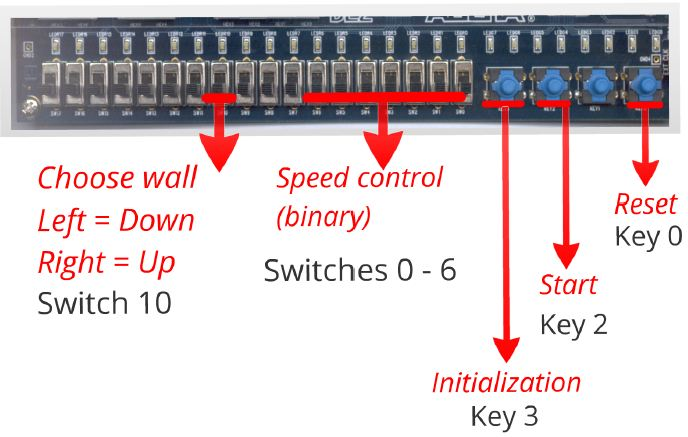
\includegraphics[width = \textwidth]{graphics/assignments.jpg}
      \cprotect \caption{Function assignments for DE2 peripherals.}
      \label{assign}
    \end{minipage}
  }
\end{figure}

The switch and button assignments on the DE2 board are shown in
Fig.~\ref{assign}.  Switches \verb+SW0+ through \verb+SW6+ are used to
encode in binary the speed at which the robot will travel. Switch
\verb+SW10+ selects which wall is to be followed, with a low value
indicating the right-wall following program.
 
To start the program, a series of steps must be followed. First, the
switches are toggled into the desired positions. \verb+KEY3+ is then
pressed to initialize the robot. Lastly, \verb+KEY2+ is pressed to
start the program. \verb+KEY0+ may be pressed at any time to reset
the program.


\subsection{Significant Modifications}

Several significant modifications were made to the original design:

\begin{itemize}
\item The original program consisted of five states. During testing it
  was discovered that the inaccuracy of sensor data when the robot was
  angled to the wall caused premature transitions to an ``outside turn'' state. To
  solve this problem, the state was removed. To navigate outside
  turns, the ``adjust inward'' state is used. A subroutine in this state
  limits the value of the lateral sensors to prevent the robot from
  turning too sharply. 
\item It was originally proposed to use the LCD display to
  show the state that the wall following program is currently
  in. However, since the LCD is not timed on the same clock as
  SCOMP, the team encountered problems timing the latching of IO
  data into the LCD when other IO peripherals,
  such as motor and sensor control, were also being used. To solve
  this problem, the role of  the LCD display was changed to display
  the basic startup states and  not the current wall following  state. 
\item The original design called for one lateral sensor \(s_5\) (or \(s_0\)) and
  one forward sensor \(s_2\) (or \(s_3\)) whose data would serve as inputs to the
  state machine. Since the sensor readings were inaccurate when the
  robot was oriented at an angle to the wall, it was decided that
  using pairs of sensors would be optimal. A pair of sensors, \(s_4\)
  and \(s_5\) (or \(s_0\) and \(s_1\)) was used for the lateral
  region, and the pair \(s_2\) and \(s_3\) for the forward region. The
  minimum value of each pair was used as the working value for the
  distance of the robot to a wall in either the lateral or forward region.
\end{itemize}


\subsection{Project Management}

The finalized Gantt chart that was used during this project can be found in Appendix~\ref{appndx}. 

\section{Technical Results}

\subsection{Final Demonstration Results}

The course used for the final demonstration consisted of five straight
wall segments, with four outside turns and four inside turns. Each
straight segment of the course was approximately four feet. 

The results of the final demonstration showing the \textbf{expected},
\textbf{actual}, and \textbf{difference}  in values of scores can be found in
Table~\ref{results}. The expected values for the completion, accuracy,
and time are based on test runs performed during lab periods. 

\begin{table}[h!]
  \centering \cprotect \fbox{
    \begin{minipage}{5.5in}
      \centering
      \small
     \cprotect \caption{Results of wall following demo}
      \label{results}
      \begin{tabular}{|c|c|c|c|c|c|c|c|c|c|}
        \hline
        &\multicolumn{3}{|c|}{\textbf{Completeness} (\%)}&
        \multicolumn{3}{|c|}{\textbf{Accuracy} (\%)}&
        \multicolumn{3}{|c|}{\textbf{Time} (min:sec)} \\ \hline
        &\textbf{Exp.}&\textbf{Act.}&\textbf{Diff.}&
        \textbf{Exp.}&\textbf{Act.}&\textbf{Diff.}&
        \textbf{Exp.}&\textbf{Act.}&\textbf{Diff.}  \\
        \hline
        \textbf{Right Wall} & 100\% & 100\% & - & 100\% & 100\% & - &
        1:15 & 1:23 & 0:08 \\ \hline
        \textbf{Left Wall} & 100\% & 100\% & - & 100\% & 0\% & 100\% &
        1:15 & 5:52 & 4:37 \\ \hline
        \multicolumn{7}{|l|}{\textbf{Total Time}} & 2:30 & 6:15 & 3:45 \\ \hline
      \end{tabular}
    \end{minipage}
  }
\end{table} 

The robot did not collide with the wall on either run. It received an
accuracy bonus for five out of the ten sections it completed. 

The robot completed the course following the right wall in one minute
and 23 seconds, which was eight seconds slower than the expected
time. The robot was 100\% accurate during this run.

The team experienced problems during the left wall following
demonstration. The problems encountered were due to the prevalence of
sequential inside turns in the particular left-wall following course
presented. One issue identified was that the robot was inconsistent in
detecting its distance to a forward wall, which is crucial to execute
an inside turn. The result was that the robot would frequently turn
too early or too late and would be unable to readjust to recover in
time for the next turn. The
problem was in the range-calculating algorithm implemented and not in the
hard-coded \(90^\circ\) turns using rotary encoder measurements, since
the turns executed were exceptionally consistent. The time to complete the
course was a result of several trial runs due to near collisions. The
robot was switched for another robot at the behest of the professor
due to strange sensor behavior on the left side. This event caused
additional setup and upload delays. The robot was able to succesfully
complete the course, but did so without maintaining a constant
distance to the wall.

\subsection{Outcomes}

The results from the final demonstration and test runs suggest that
the robot can consistently and accurately complete a wall following
course predominantly composed of outside turns. When performing
sequential inside turns, the robot is often unable to successfully
navigate the course. In either case, the robot must travel very slowly
to avoid collisions with the wall. 







\section{Conclusions}

\subsection{Overview}

Overall, the design allowed the robot to successfully complete the
course. The design met all specifications. However, maintaining a
constant distance to the wall proved to be a challenge. While the
robot did not have problems maintaining accuracy when following the
right wall, it was unable to produce the same results when following the
left wall. Accuracy on the right wall following depended strongly on
suppressing the speed of the robot. The robot completed both courses
without collisions and penalties. 

\subsection{Strengths and Weaknesses of Design}

There are several strengths of this design. The robot is able to
successfully complete the course and avoid collisions. The design
allows the robot to run at variable speeds chosen by the user by
selecting switches on the DE2 board. The informative display greatly
helps in debugging processes and provides insight into how the program
is running. 

A weakness of this design is that the Amigobot cannot utilize its
speediness and complete the course successfully without
collisions. Extra time, in the form of slow movement, must be used in
order to accurately follow the wall. Additionally, the algorithm
itself is inefficient and produces inconsistent results. The
inefficiency stems from the multiple 100  ms wait loops in the adjustment states that
slow down sensory input tremendously. Wall following inconsistency may be attributed to
an inflexible algorithm unable to handle sensor inaccuracies.

\subsection{Recommendations}

For future work, a useful development would be to show the moving
states on the LCD display as initially proposed. This would allow for quicker and more
effective debugging and would be a useful addition to the display. 

Another development would be to encode the green LEDs to show more
functions as they are executed. The current design uses the green LEDs
only as a completion bar for the ``inside turn'' state. Animating the LEDs
for other states could aid in debugging purposes and improve the
display. 

While this design takes the minimum of two adjacent sensory values, it
could be edited to use weighted values of the sensors. Allowing some
sensors to take precedence over others would allow the robot to
accurately determine its orientation relative to the wall. 

Due to limited computational resources in assembly language, the
measurement algorithm used to detect turns is not as accurate as
desired. A major improvement to the program would be to compute a more
accurate measurement algorithm, such as averaging the forward sensor
data over multiple instances of time.

\subsection{Optimizations}

In order to optimize the design, the 100 ms wait loops should be removed
from the adjustment states. The loops decrease the frequency of adjustment
greatly, which prevents the robot from moving too quickly. In order to
remove the wait loops, the adjustment states would have to be
rewritten in order to remove cumulative additions. 

Additionally, the invalid value of the sonar sensors should be changed
from \verb+0xFFFF+ (\(-1\)) to a large positive number,
\verb+0x7FFF+ (32767). Since the code implemented includes many \verb+JNEG+
instructions, this would prevent having to include special
consideration for invalid sensor readings. Ideally, this would be
changed at the hardware level of the sonar sensors. 
\titleformat{\section}{\LARGE\bfseries}{\appendixname\:\thesection:}{1em}{}{}

\newpage
\begin{appendices}
%\appendixtitleon
%\appendixname
\section{Gantt Chart} \label{appndx}
\begin{center}
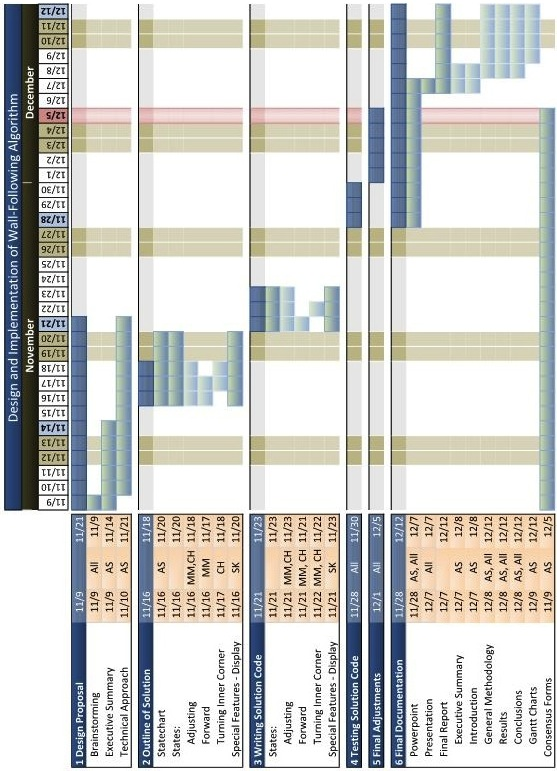
\includegraphics[height = 8in]{graphics/gantt_chart}
\end{center}


\newpage
\thispagestyle{empty}
\section{Logbook}
\newpage
\thispagestyle{empty}
\section{Design Proposal}\label{proposal}
\end{appendices}


%\bibliographystyle{IEEEtran}
%\bibliography{IEEEabrv,bib-1}

\end{document}



%\begin{figure}[h!]
%\centering
%\cprotect \fbox{
%\begin{minipage}{6.5in}
%\centering
%\includegraphics[width =  \textwidth]{img_here}
%\cprotect \caption{}
%\end{minipage}
%}
%\end{figure}

